\documentclass[a4paper,titlepage]{article}
\usepackage{frontespizio}
\usepackage[italian]{babel}
\usepackage[utf8]{inputenc}
\usepackage{usecases}
\usepackage{listings}
\usepackage{verbatim}
\usepackage{tikz}
\usetikzlibrary{arrows,shadows} % for pgf-umlsd
\usepackage[underline=true,rounded corners=false]{pgf-umlsd}

\usepackage{enumitem}
\setitemize{noitemsep,topsep=0pt,parsep=0pt,partopsep=0pt}

\usepackage[a4paper, total={6in, 9in}]{geometry}

\lstset {
basicstyle=\small,
escapeinside=\`\`,
breaklines=true
}


\begin{document}
\begin{frontespizio}
\Universita{Verona}
\Dipartimento{Informatica}
\Corso[Laurea]{Informatica}
\Titoletto{Basi di Dati}
\Titolo{Elaborato}

\Candidato[VR359169]{Enrico Giordano}
\Candidato[VR361121]{Cristian Pinna}

\Annoaccademico{2013-2014}
\end{frontespizio}

\tableofcontents

\newpage

\part{Progettazione Concettuale}

\vfill
    \begin{center}
	
\centerline{
    %\centering
    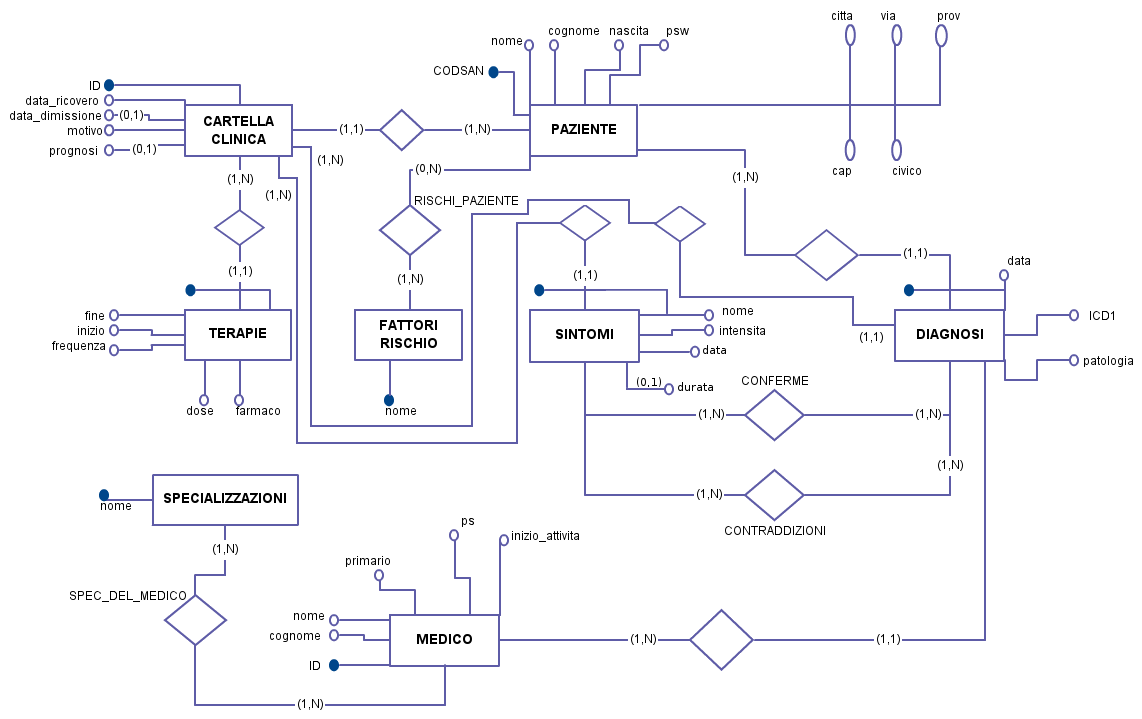
\includegraphics[scale=0.45]{ER.png}
}
    \end{center}
\vfill
\newpage
{\large Elenco delle relazioni:}\newline

\begin{enumerate}

\item Relazione TERAPIE - CARTELLA CLINICA:

\begin{itemize}[leftmargin=0.5cm, topsep=0.25cm, itemsep=0.2cm]

\item Cardinalità (1,1), una TERAPIA è associata univocamente ad una CARTELLA CLINICA
\item Cardinalità (1,N), ad una CARTELLA CLINICA può corrispondere più TERAPIE

\end{itemize}

\item Relazione CARTELLA CLINICA - PAZIENTE:

\begin{itemize}[leftmargin=0.5cm, topsep=0.25cm, itemsep=0.2cm]

\item Cardinalità (1,1), una CARTELLA CLINICA è associata univocamente ad un PAZIENTE
\item Cardinalità (1,N), ad un PAZIENTE può corrispondere più CARTELLE CLINICHE

\end{itemize}

\item Relazione CARTELLA CLINICA - SINTOMI:

\begin{itemize}[leftmargin=0.5cm, topsep=0.25cm, itemsep=0.2cm]

\item Cardinalità (1,N), ad una CARTELLA CLINICA può corrispondere uno o più SINTOMI
\item Cardinalità (1,1), un SINTOMO è associato univocamente ad una CARTELLA CLINICA

\end{itemize}

\item Relazione CARTELLA CLINICA - DIAGNOSI:

\begin{itemize}[leftmargin=0.5cm, topsep=0.25cm, itemsep=0.2cm]

\item Cardinalità (1,N), ad una CARTELLA CLINICA può corrispondere una o più DIAGNOSI
\item Cardinalità (1,1), una DIAGNOSI è associata univocamente ad una CARTELLA CLINICA

\end{itemize}

\item Relazione PAZIENTE - FATTORI RISCHIO:

\begin{itemize}[leftmargin=0.5cm, topsep=0.25cm, itemsep=0.2cm]

\item Cardinalità (0,N), ad un PAZIENTE può corrispondere nessuno o più FATTORI RISCHIO
\item Cardinalità (1,N), ad un FATTORE RISCHIO può corrispondere uno o più PAZIENTI

\end{itemize}

\item Relazione PAZIENTE - DIAGNOSI:

\begin{itemize}[leftmargin=0.5cm, topsep=0.25cm, itemsep=0.2cm]

\item Cardinalità (1,N), ad un PAZIENTE può corrispondere una o più DIAGNOSI
\item Cardinalità (1,1), una DIAGNOSI è associata univocamente ad un PAZIENTE

\end{itemize}

\item Relazione SINTOMI - DIAGNOSI:

\begin{itemize}[leftmargin=0.5cm, topsep=0.25cm, itemsep=0.2cm]

\item Cardinalità (1,N), ad un SINTOMO può corrispondere una o più DIAGNOSI
\item Cardinalità (1,N), ad una DIAGNOSI può corrispondere uno o più SINTOMI

\end{itemize}

\item Relazione DIAGNOSI - MEDICO:

\begin{itemize}[leftmargin=0.5cm, topsep=0.25cm, itemsep=0.2cm]

\item Cardinalità (1,1), una DIAGNOSI è associata univocamente ad un MEDICO
\item Cardinalità (1,N), ad un MEDICO può corrispondere una o più DIAGNOSI

\end{itemize}

\item Relazione MEDICO - SPECIALIZZAZIONI:

\begin{itemize}[leftmargin=0.5cm, topsep=0.25cm, itemsep=0.2cm]

\item Cardinalità (1,N), ad un MEDICO può corrispondere una o più SPECIALIZZAZIONI
\item Cardinalità (1,N), ad una SPECIALIZZAZIONE può corrispondere uno o più MEDICI

\end{itemize}

\end{enumerate}

\newpage

\part{Schema Logico}
    \begin{center}

    \centering
    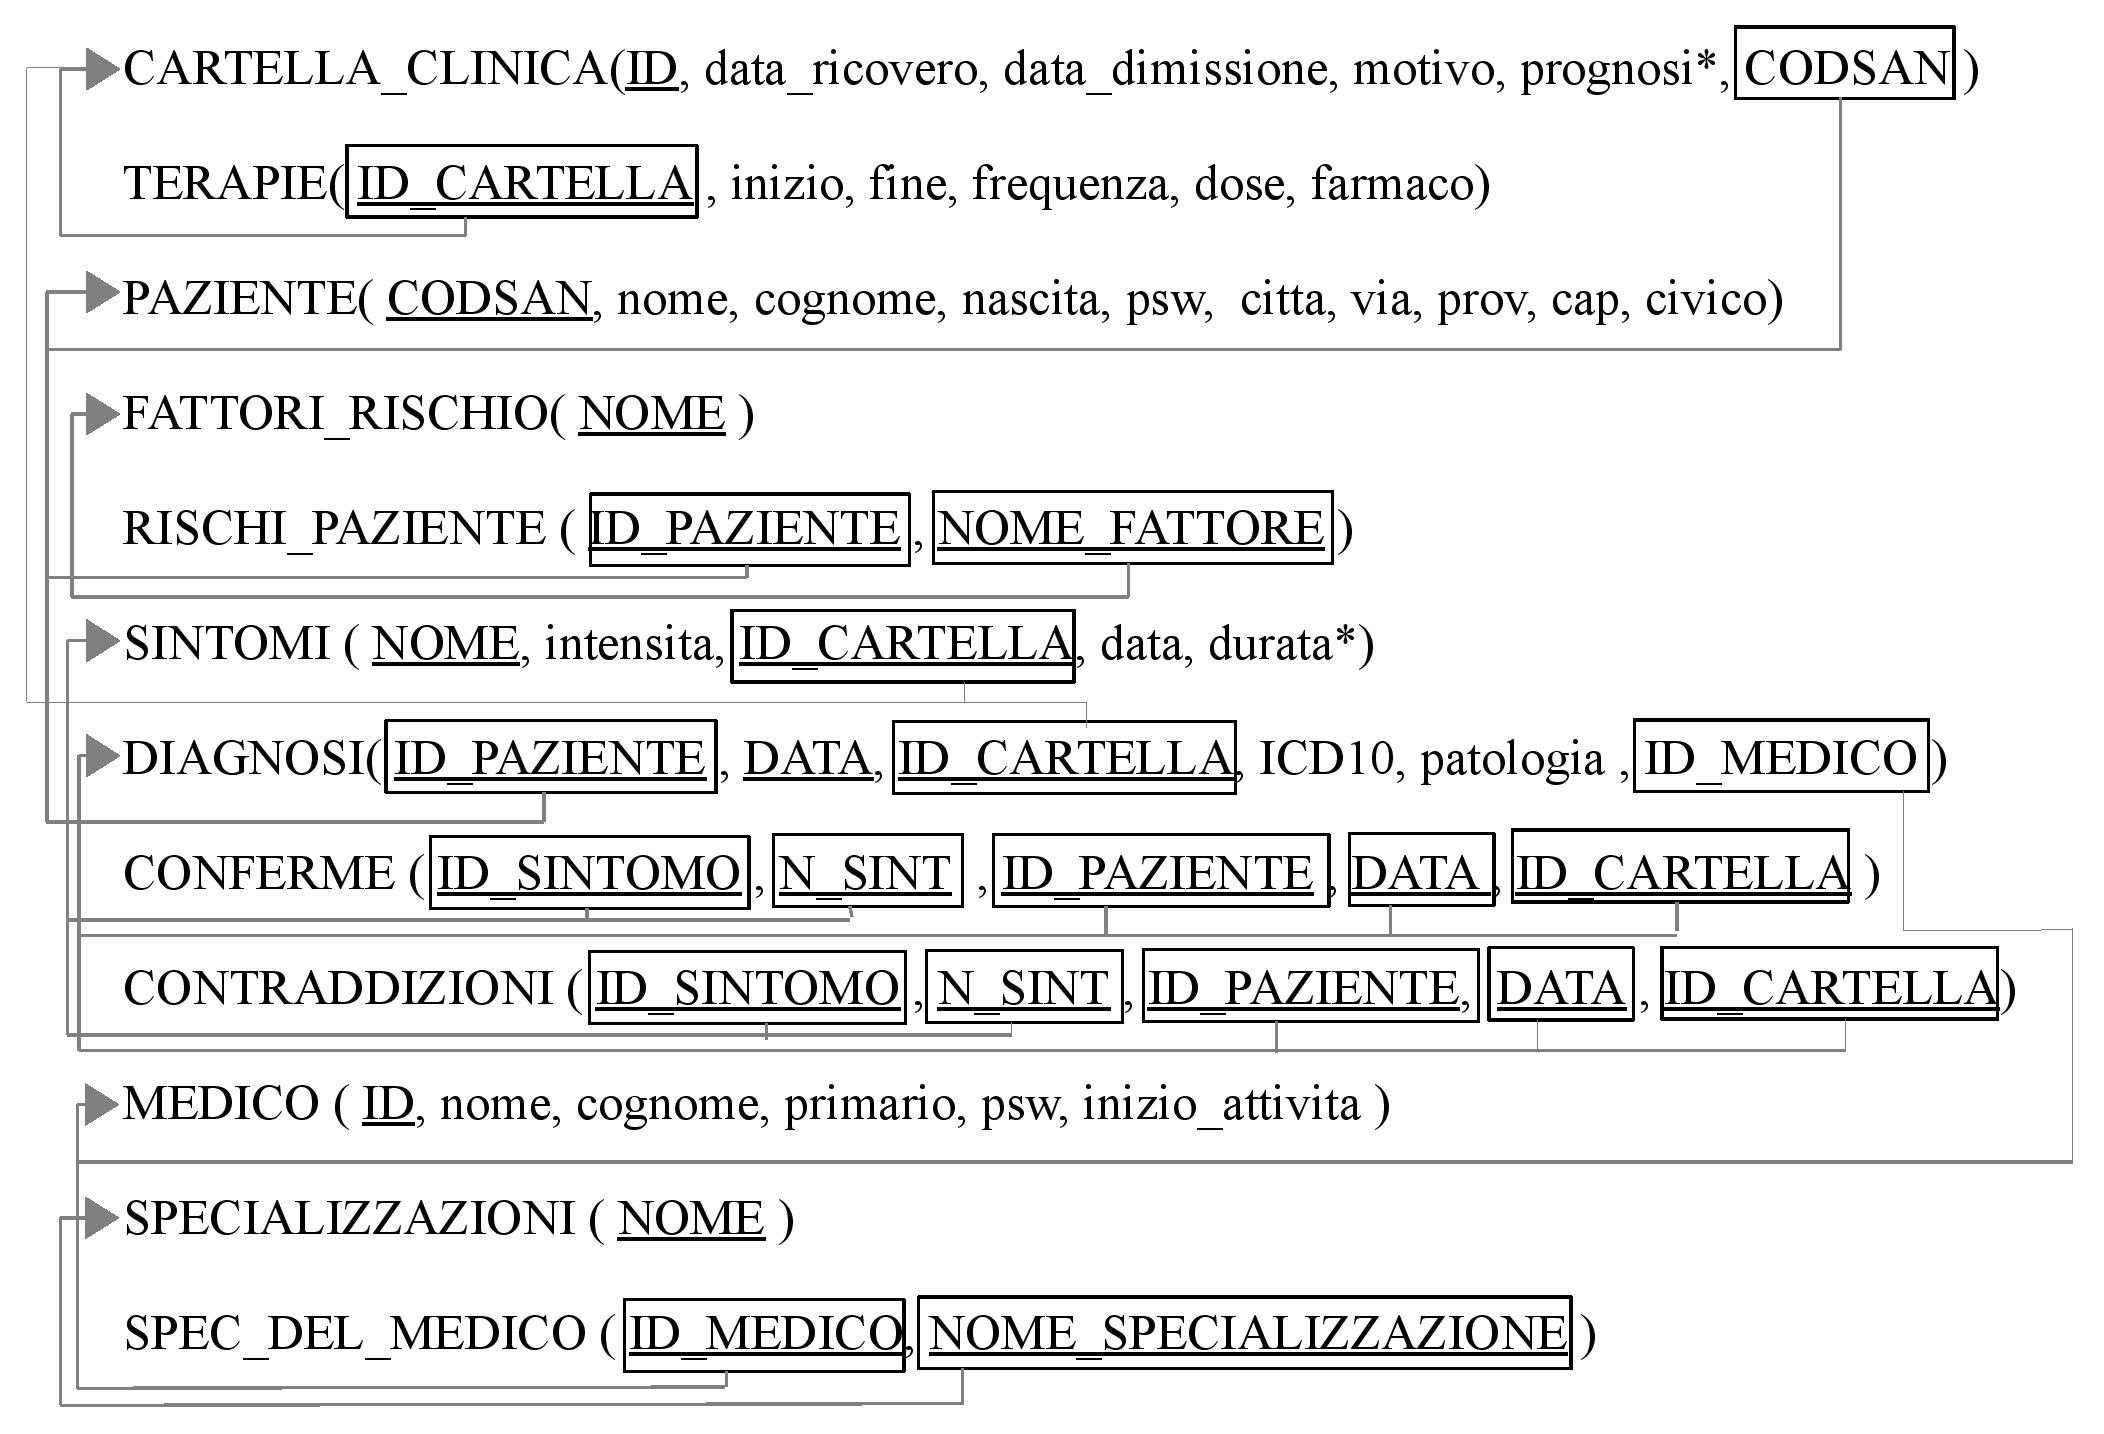
\includegraphics[scale=0.9]{schema_logico.jpg}

    \end{center}

Questo schema logico rappresenta una visione globale sull'elenco dei vari attributi, sulle chiavi primarie (attributi sottolineati) e sulle relazione tra di essi (i riquadri attorno al nome dell'attributo e la relativa freccia che punta alla relazione).
\newpage
\part{Page Schema}
\begin{lstlisting}
`\textbf{page-schema Homepage unique (}`
	presentazione: string;
	foto_divisione: image;
	primario: string;
	login_paziente: form(
		login:text;
		pw: password;
		invia: submit();
	);
	personale_medico: link (personale, *PatologieLink);
	login_medico: form(
		login: text;
		pw: password;
		invia: submit();
	);
`\textbf{);}`

`\textbf{DB to page-schema HomePage (}`
	primario: select nome, cognome from primario;
	login_cliente:
		if(	select codsan
			from paziente
			where login = ? and pw = ?)
		then *PazientePage else *HomePage
		end;
	login_medico:
		if(	select id
			from medico
			where login = ? and pw = ?)
		then *DiagnosiPage else *HomePage
		end;

`\textbf{page-schema PazientePage  (}`
	dati: list of (
		codice_sanitario: string;
		nome: string;
		cognome: string;
		data_nascita: string;
		via: string;
		civico: string;
		cartella_clinica: link(cartella clinica, *CartellaPage);
		fattori_rischio: string;
	);
	elenco_medici: list of(
		nome: string;
		cognome: string;
	);
`\textbf{);}`

`\textbf{DB to page-schema PazientePage (}`
	dati: 	select paziente.*
		from paziente
		where codsan = ?;
	cartelle_cliniche: list of(
		id_cartellaclinica: link(cartella clinica, *CartellaPage);
	);
	elenco_medici:	select []
			from paziente, []
			where codsan = ?;
`\textbf{);}`		

`\textbf{page-schema CartellaPage (}`
	ID: string;
	dataRic: string;
	motivo: string;
	prognosi: string;
	nome_medico: string;
	cognome_medico: string;
`\textbf{);}`

`\textbf{DB to page-schema CartellaPage (}`
	dati:	select cartellaClinica.*, medico.nome, medico.cognome
		from  cartellaClinica, medico
		where [];
`\textbf{);}`

`\textbf{page-schema PatologiePage (}`
	patologie: text;
`\textbf{);}`

`\textbf{DB to page-schema PatologiePage (}`
	patologie: 	select *	
			from patologia, paziente
			where [];
`\textbf{);}`

`\textbf{page-schema PersonalePage (}`
	dati: text;
`\textbf{);}`

`\textbf{DB to page-schema PatologiePage (}`
	dati: 	select medico.*, count(diagnosi)
		from  medico, diagnosi
		where [];
`\textbf{);}`

`\textbf{page-schema PersonalePage (}`
	new_diagnosi: form (
		data: string;
		paziente: string;
		ICD10: string;
		sintomi: list of (string); //radio button per dire se e' una conferma o una contraddizione
	);
`\textbf{);}`

`\textbf{DB to page-schema PersonalePage (}`
	new_diagnosi: INSERT INTO DIAGNOSI VALUES (?paziente?, ?data?, 
		      ?sintomo?, idMedico);
		      INSERT INTO CONFERME || INSERTO INTO CONTRADDIZIONI	
`\textbf{);}
}
\end{lstlisting}
\newpage
\begin{comment}
\part{General pattern}

Now we explain an example of system behaviour: when a car arrives or exits to the park, the node ''car detector`` sends a message to the node ''process unit``, that store the request (for future use) and send to the monitor the average number of car/hour and the number of free parking places.

According to observer pattern, the subject (Sensor) notify the observer (Process Unit) that a new message is pending, so the observer (Process Unit) receive istantly the message. After the computation, in the same the Process Unit send messages to the different displays.
The observer pattern is used only in the comunication nodes.

So when the sender node has to send a message , it must call the receive method of the receiver node; in this way it's implemented an observer pattern, which is an optimization of a real system. In fact, in a real context, the receiver must poll on the receive path (or hardware) or must have an interrupt routine that manage the receiving process; in this system, the sender calls the ``receive`` method of the receiver.

In the picture, the arrows show how a class (or a method) call other class (a class is called to another class).

    \begin{center}

    \centering
    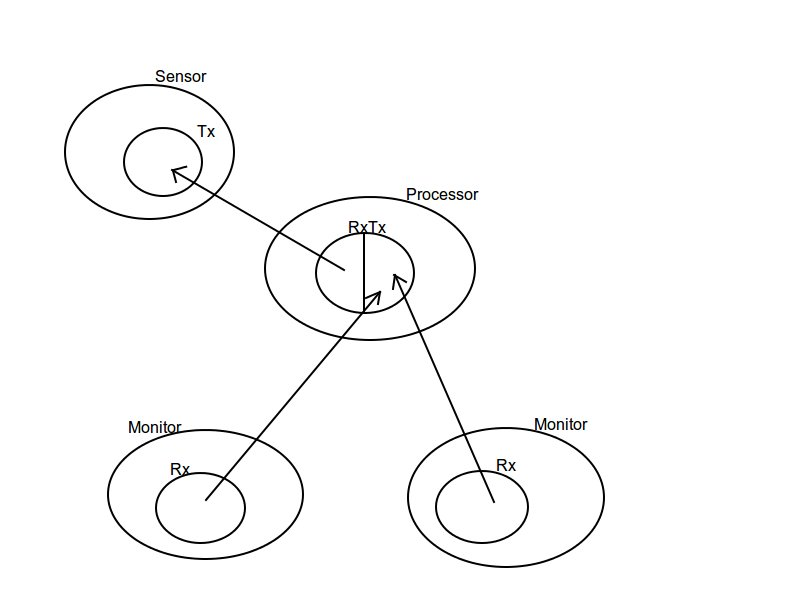
\includegraphics[scale=0.40]{pattern.jpg}

    \end{center}


The ``abstract`` class Node is implemented in the following classes

\begin{itemize}[noitemsep,topsep=20pt,parsep=10pt,partopsep=20pt]

\item Detector: a sensor that controls car traffic (entering or exiting car);
\item Processor: a processing unit that calculate average number of cars/hour and number of free parking places;
\item Monitor: a display that shows the results of processing unit.

\end{itemize}

The channel comunication is implemented by ``Channel`` class, that create a link in a comunication grid. There are 2 types of Channel: WireChannel and WirelessChannel (in this project there is no difference).

All the operations in the Processor are implemented by other classes that implement basic operation (sum, min, ecc...). These classes extend NodeComputation interface. A complex computation is formed by a combination of basic operations, like an ALU in a real processor.

The NodeCommunication interface manages the exchange of messages between nodes and is implemented in the following classes:

\begin{itemize}[noitemsep,topsep=20pt,parsep=10pt,partopsep=20pt]

\item TxNode: must send a message (for Detector);

\item RxNode: must receive a message (for Monitor);

\item TxRxNode: must send and receive a message (for Processor);

\end{itemize}

\newpage
\part{Simulation}

The detector, the processing unit and 3 monitors are created in the main class. These monitors show a display for average number of car/hour, a display for number of free parking places and a (not required) display for car traffic.

The nodes are linked in the wireless grid so they can comunicate one another. A realtime clock in the processing unit simulates the time (for the average cars/hours) implemented with a thread that increase a counter every second.

\section*{GUI}

In according to show a simulation of the system we have implemented a simple user interface. There are:

\begin{itemize}

\item a control button panel, which contains three buttons (start, stop, reset) that controll intuitively the system;
\item a complex of simple monitor that show the evolution of the system.

\end{itemize}

The user can control the simulation with some control buttons: the ``start'' button starts the simulation, the ``stop'' button stops the simulation and the ``restart'' button restarts the simulation.

    \begin{center}

    \centering
    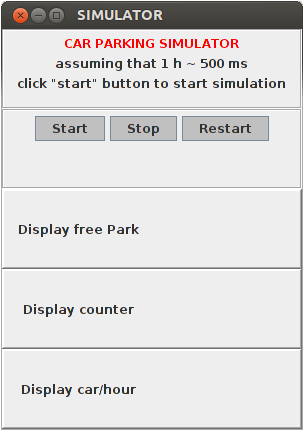
\includegraphics[scale=0.50]{interface.png}

    \end{center}

 
\newpage
\part{Questions}

\section*{ Which patterns are used within the scheme of Figure 2?}

The first figure represents an interface class called ``nodeCommunication'' and three other classes (TxNode, RxNode and TxRxNode) that implement the nodeCommunication interface. The interface class is a type of class that presents many methods of a particular class; this methods are not implemented, but the class that implements this interface must implements them.

~

The second figure represents an another interface called ``nodeComputation'' and some other classes (Add, Sub, Average, Divide, Multi, Comparator) that implement nodeComputation interface. Every nodeComputation class must have a method that must be implemented by the programmer. Interfaces cannot be instantiated, but rather are implemented. A class that implements an interface must implement all of the methods described in the interface, or be an abstract class. They simulate multiple inheritance.

~

The third figure represents an abstract class called ``Node'' and three other classes (Detector, Processor, Monitor) that inherited the superclass methods (``Node''). The abstract class must have some implemented methods and the son classes have the same method and the same attribute. If a son classes have a different implementation of a method, it must override it.

An abstract type may provide no implementation, or an incomplete implementation. Abstract types will have one or more implementations provided separately, like in this case.

~

So this is a Strategy Pattern. The strategy pattern is a software design pattern that enables an algorithm's behavior to be selected at runtime. For instance, a class that performs validation on incoming data may use a strategy pattern to select a validation algorithm based on the type of data, the source of the data, user choice, or other discriminating factors. These factors are not known for each case until run-time, and may require radically different validation to be performed. The validation strategies, encapsulated separately from the validating object, may be used by other validating objects in different areas of the system (or even different systems) without code duplication.

\newpage
\end{comment}
\part{Strategie progettuali e considerazioni personali}

Considerazioni personali e strategie adottate durante lo sviluppo del progetto:

\begin{itemize}[leftmargin=1.5cm, topsep=0.5cm, itemsep=0.2cm]

\item Realizzazione del DB in modo tale da poter ottenere più relazioni possibili con la cartella clinica;
\item Utilizzo del metodo Hibernate durante la realizzazione del progetto in modo tale da poter semplificare le query, tenendo presente che esse restituivano tanti valori nidificati a cui ci si poteva raggiungere tramite superchiavi;
\item Durante la creazione della pagina relativa alle diagnosi (DiagnosiPage) il campo delle cartelle cliniche viene popolato tramite uno script ajax-json-jquery a seconda del paziente selezionato, in modo tale da evitare l'inserimento manuale di una cartella clinica potenzialmente errata;
\item Per la realizzazione generale della pagina web che gestisce l'intero progetto ci siamo sentiti di renderla più gradevole graficalmente inserendo uno stile di impaginazione html in formato css;
\item ECLIPSE pls!

\end{itemize}

\end{document}


